\section{Camera theory}

An image captured through a camera is the result of reflected light being detected on a camera sensor, see figure \ref{fig:light_cam}. This process is know as \textit{image acquisition} and is generally not something you think about when you capture an image with a camera, since it all happens automatically. In this chapter the basics of image acquisition using a digital camera will be explained. To understand how this works it is necessary to have a basic understanding of the physics behind light.

\begin{figure}[htbp] 
\centering 
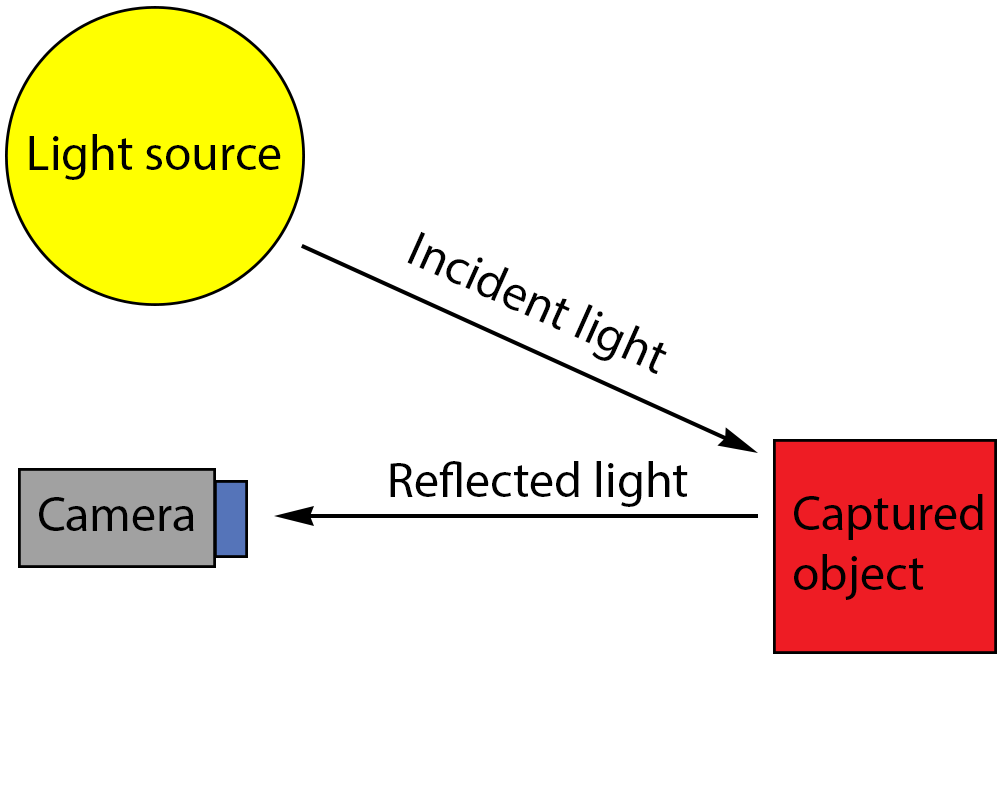
\includegraphics[width=0.5\textwidth]{Pictures/Theory/light_from_sun.png} 
\caption{Light as captured by a camera} 
\label{fig:light_cam} 
\end{figure}

Light is a form of electromagnetic radiation and can be viewed as both waves and particles. This duality is however not something that will be covered within this chapter; the wave model is sufficient to build the foundation of the understanding we need. A light wave is a small packet of energy travelling through space. These energy packets are known as photons. Photons can be described by three properties:

\begin{itemize}
\item \textbf{Wavelenght} - Measured in meters from wave top to wave top and denoted as $\lambda$.
\item \textbf{Frequency} - Measured in oscillations per second, Hz, denoted $f$.
\item \textbf{Energy} - Measured in electronvolts, eV, denoted $E$.
\end{itemize}

The formulae for these properties are as follows:
To derive the wavelength or the frequency, formula \ref{eq:wavelenght} is applied:
\begin{align}
\centering 
\lambda = \frac{C}{f}
\label{eq:wavelenght} 
\end{align}
$\lambda$ and f we are familiar with, and C is the speed of light. The second equation, equation \ref{eq:e_v}, describes the energy:
\begin{align}
\centering
E = \frac{hC}{\lambda}
\label{eq:e_v} 
\end{align}
Where h is Planck's constant, which describes the proportional relationship between energy of a photon and an the corresponding electromagnetic waves frequency. E, C and $\lambda$ are still as explained above.

The wavelength of the photon determines what color one perceives. However, as known from physics, the speed of light is constant; thus changing the frequency will alter the wavelength and therefore the color that is perceived. The visible spectrum of light is but a fraction of the full spectrum of electromagnetic radiation, see figure \ref{fig:em_rad}. Light interacts additively, with a mix of equal parts of each wavelength resulting in white light. The most common light source is the sun. The white light from the sun can be broken down into its component wavelengths by refracting the light in a prism. This will yield the full spectrum of visible light, as seen in a rainbow.
While different wavelengths correspond to different colors, these colors only remain defined within our perception. The reason we see ~600 nm light as yellow is because our eyes contain three types of optically sensitive cells, known as \textit{cones}, constructed to be sensitive to three colors: red, green and blue. 600 nm lies between the green and red cells, thus both cells are firing and the perceived color becomes yellow.\citep{perception_book}.

\begin{figure}[htbp] 
\centering 
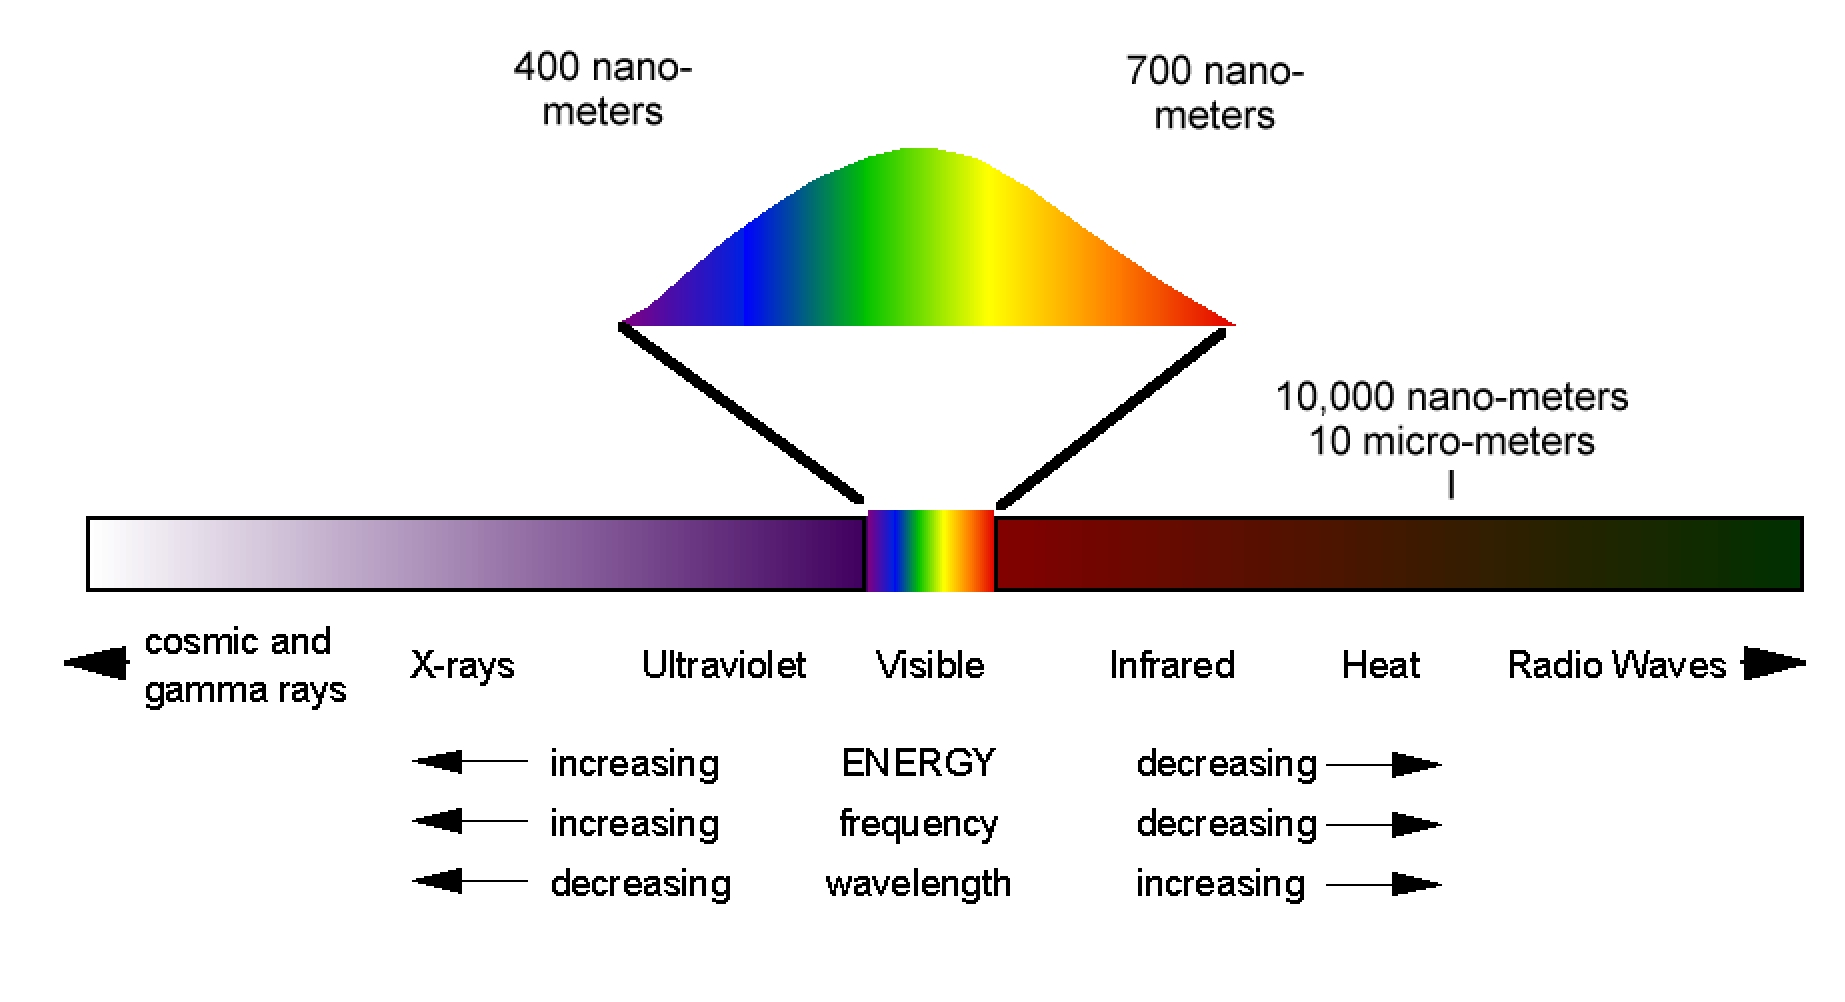
\includegraphics[width=1\textwidth]{Pictures/Theory/em_rad.png} 
\caption{The full spectrum of electromagnetic radiation.} 
\label{fig:em_rad} 
\end{figure}

\subsection{Digital image acquisition}
When capturing an image using a digital camera, light is passed through a lens onto the sensor, which acts in much the same way as the human eye. In place of cones sensitive to specific wavelengths, a camera sensor has a physical matrix of pixel sensors, one for each pixel in the output image. A camera that can only capture black and white images has only one type of sensor in each physical pixel whereas a camera that captures color images has three types of sensors in each pixel \citep{ip_book}.

\subsection{Image acquisition in the project}
In the project, two cameras were considered: a normal RGB webcam and a similar camera with an infrared (IR) filter installed. The filter consists of a small strip of normal analogue film, used for analogue pictures, that has been mounted on the lens. The film strip allows only infrared light to pass, thus making the only light that reaches the sensor infrared.

\begin{figure}[htbp] 
\centering 
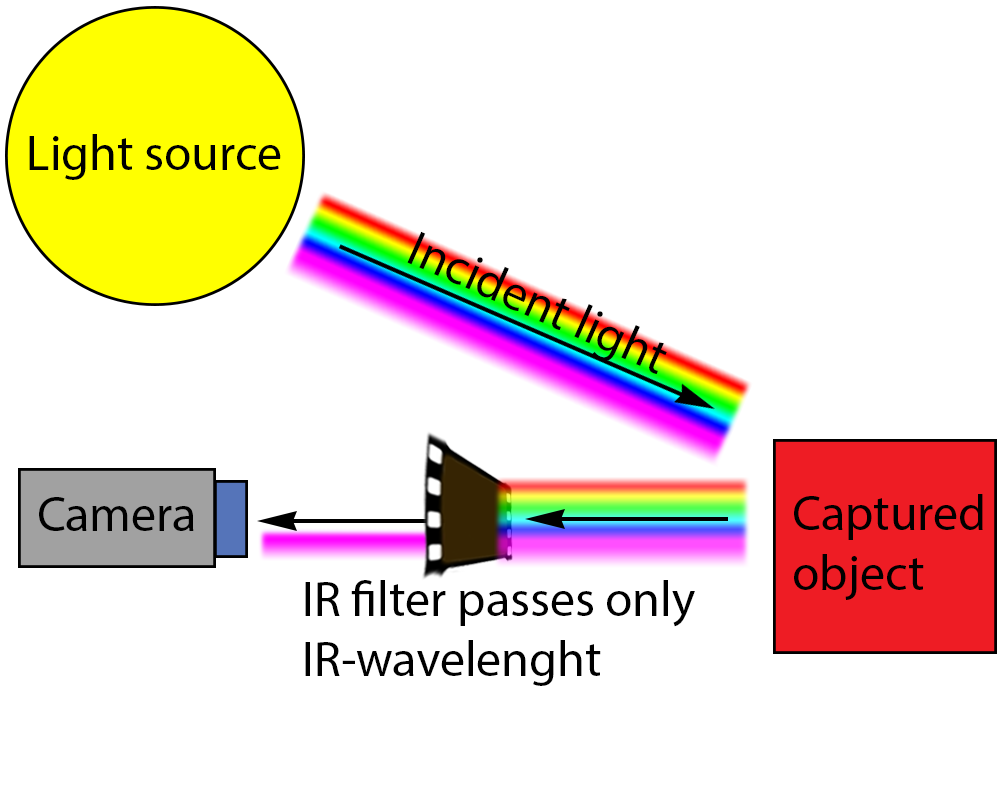
\includegraphics[width=0.5\textwidth]{Pictures/Theory/IR_filter.png} 
\caption{The IR filter only allows infrared light to pass.} 
\label{fig:ir_filter} 
\end{figure}

This is interesting, as it enables a larger degree of control over the illumination in the scene that is captured. Normally in a scene, controlling the lighting can prove a challenge, and in order to operate without error an image processing algorithm would have to take into account the variance in lighting that occurs naturally during a day cycle. \citep{ip_book} Working with infrared light eliminates this issue.

\subsection{Infrared light}

Infrared light lies right next to visible light in the electromagnetic spectrum, see figure \ref{fig:em_rad}. Infrared light can be used to illuminate things without having a visible component to the light, but this requires a device capable of capturing IR. Some, generally cheaper, cameras are able to do this. A camera is designed to capture what a human eye can see, so in more expensive cameras infrared light is filtered out.


\subsection{Illuminating the scene}

It is important that the lightning in the scene is constant. Imagine that the scene is captured with a normal webcam: this creates an RGB image (see figure \ref{fig:scene_light}). In this case, we imagine a program that is intended to find the shelves. In order to speed things up, the image is converted to grayscale. In the right picture the program can easily find the shelves, but in the picture on the left, the program cannot find the shelves, see figure \ref{fig:scene_thresholded}.

\begin{figure}[htbp] 
\centering 
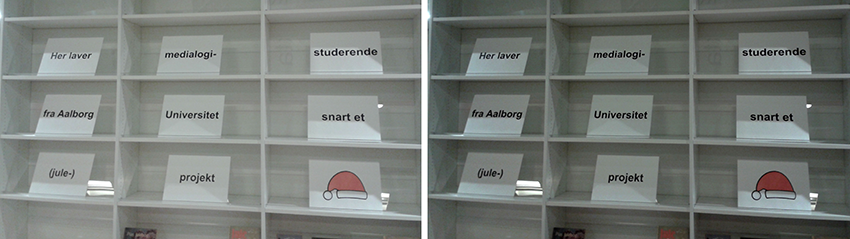
\includegraphics[width=0.5\textwidth]{Pictures/HjoerringLibrary/scene_lighting.png} 
\caption{The difference in illumination on different times of day is clearly visible when compared next to each other} 
\label{fig:scene_light} 
\end{figure}

\begin{figure}[htbp] 
\centering 
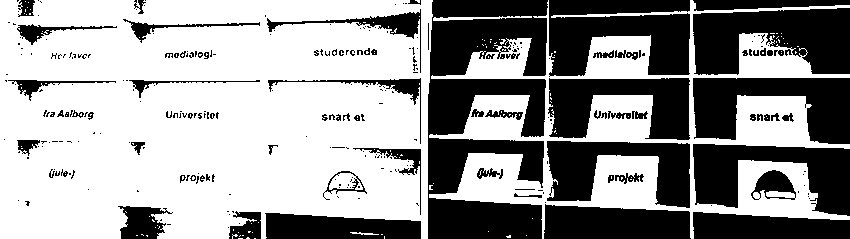
\includegraphics[width=0.5\textwidth]{Pictures/HjoerringLibrary/scene_lighting_thresholded.png} 
\caption{The same image converted to 8bit grayscale and thresholded.} 
\label{fig:scene_thresholded} 
\end{figure}

To avoid running into issues with variances in illumination, the decision was made to illuminate the scene artificially. Different options were evaluated for the illumination, all under the consideration that we had the ability to filter the camera input, allowing only infrared light to pass to the camera. The following options were considered:

\begin{itemize}
\item Using the library's lighting.
\item Making adjustments to the lighting at the library.
\item Bringing normal lights to light the scene.
\item Building our own light system to light the scene.
\end{itemize}

\subsubsection{Using the library's lighting}
The library's lightning consist of two different types of lamps: fluorescent lights, and very bright halogen spots. Using the infrared camera, we looked at the normal lighting and the halogen spots radiated too much IR light for us to be able to have a decent contrast between background and the subject we want to track.

\subsubsection{Making adjustments to the lighting at the library}
It was not possible to adjust the fluorescent lights, but the halogen spots could be pointed in a different direction. We further considered using some material to direct the cone of light from the spots, as to create the largest contrast between background and subject. Two options presented themselves: point the lights at the background, or point the lights to the subjects. These two cases offer two different problems. Limiting the cone of the light to only hit the subjects would require the light to be incident from a angle where they could not be placed, on the other hand limiting the spots to illuminating the canvas would interfere with the projection of images, as the spots are very bright.

\subsubsection{Bringing normal light to the scene} 
By bringing normal lights that emit a high amount of IR lighting, the subject could be illuminated in a sufficient manner, but this would require a mount to be created or bought.

\subsubsection{Building our own light system to light the scene}
Building a lighting system from scratch to light the scene would allow a tailored solution for the installation, removing the problems offered by the other solutions. By having a strip of bright infrared lights, and using this to light up the background, we should be able to create a high contrast between the background and the subject that we want to track. Furthermore, this provides us with the added benefit of already having defined a region of interest, thus easing the workload of the image processing.

\subsection{Concluding on the setup}
Using the default setup at the library did not provide a decent scene to be captured and processed by the program. The lights at the library were too diffuse, making adjustments to the lighting still presented a problem. While the light could be controlled to only illuminate the background, the visible light emitted would shine too bright, making the image from the project hard to make out. Bringing normal lights result in the same problem. This meant that the final decision was to create a custom infrared lighting for the library.

\section{building the LEDs}
For illuminating the scene, several different alternative were discussed and ultimately IR LEDs were chosen \fxnote{Refer to the chapter in which this is discussed} because of their good illumination outside of the visible spectrum. For the project two different LEDs were tested, both emitting at roughly 880nm \citep{5mm_led} \citep{3mm_led}. A 5mm with a cone of light of 16 degrees\fxnote{source is datasheet} and a 3mm with a cone of light of 130 degrees\fxnote{source is datasheet}.

During initial testing the focussed beam from the 5mm LED looked as though it might be too focussed, making it  difficult to create a bright line of unbroken illumination. For that reason a series of experiments were conducted: A setup that tested the light that the two LEDs offered were constructed and it was apparant that the broader LEDs did not focus the light enough, and thus did not create a high enough illumination, see figure \ref{fig:5_mm_test} and \ref{fig:3_mm_test}. Therefore the choice was made to go with the 5mm, 16 degree LEDs.

\begin{figure}[htbp] \centering
\begin{minipage}[b]{0.45\textwidth} \centering
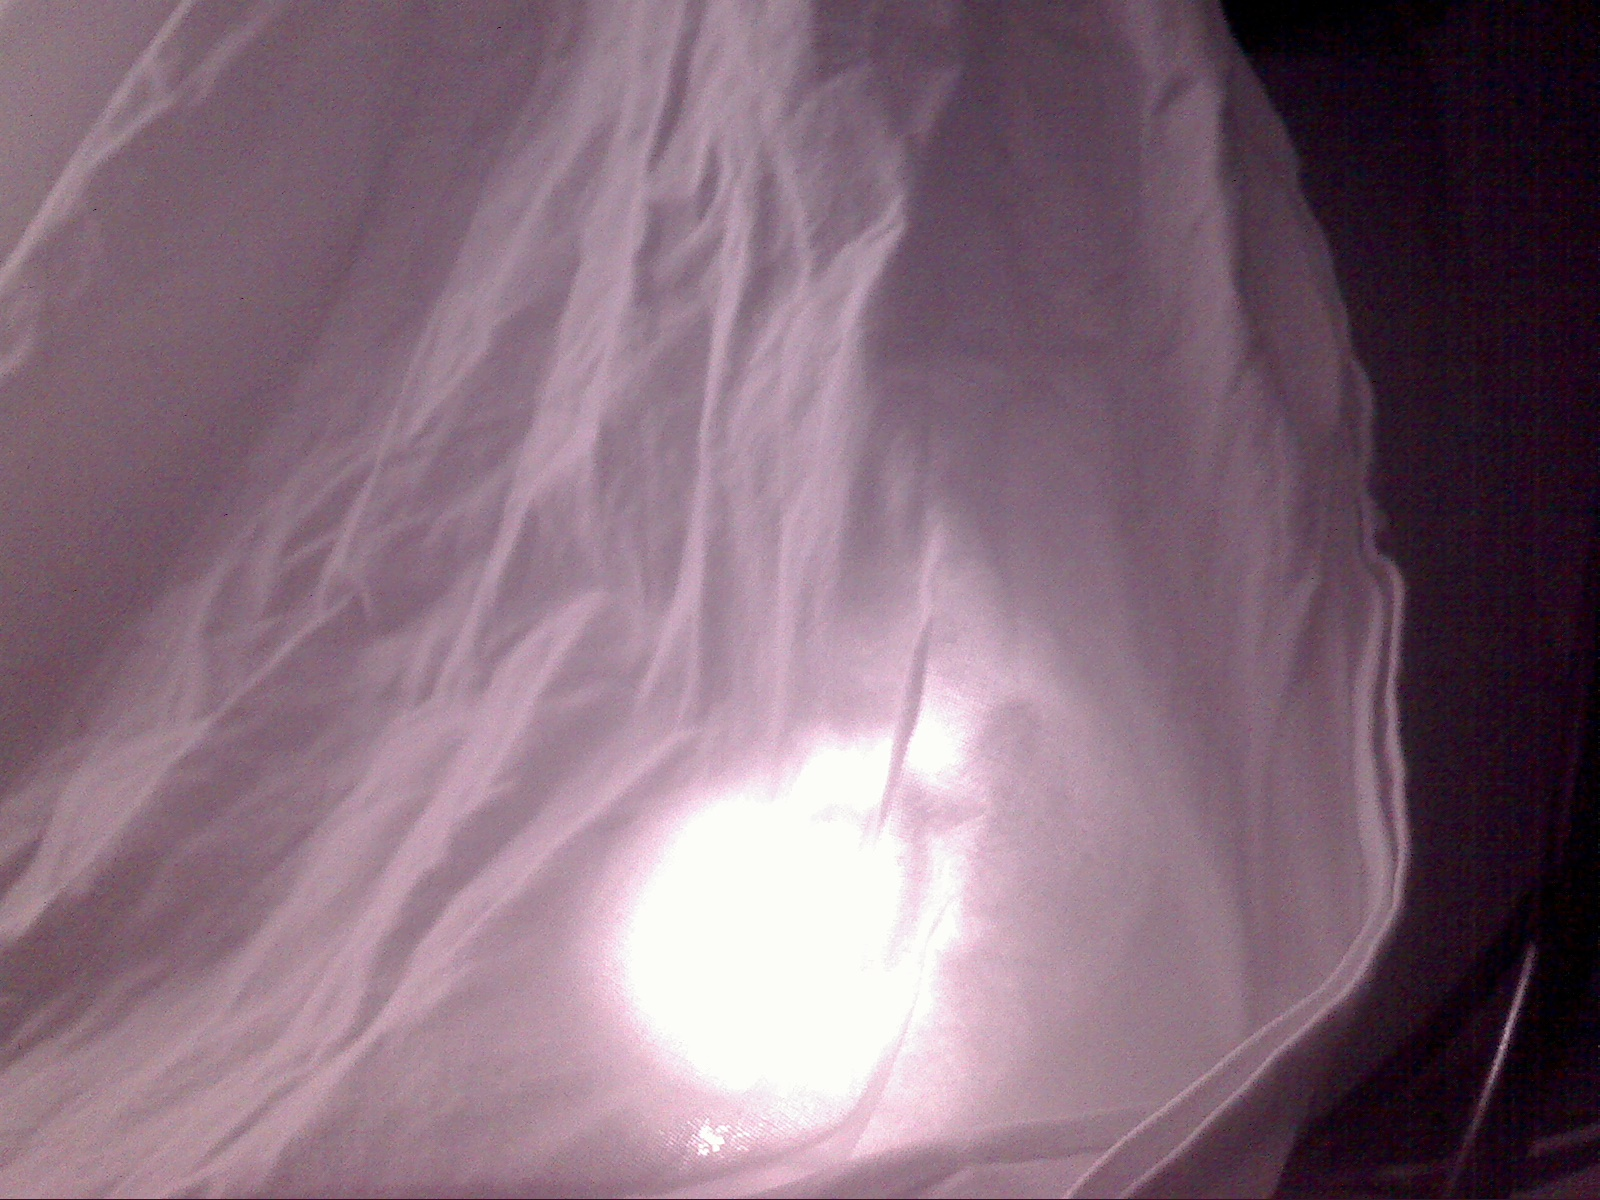
\includegraphics[width=1.00\textwidth]{Pictures/Theory/5mm.jpg} % Venstre billede
\end{minipage} \hfill
\begin{minipage}[b]{0.45\textwidth} \centering
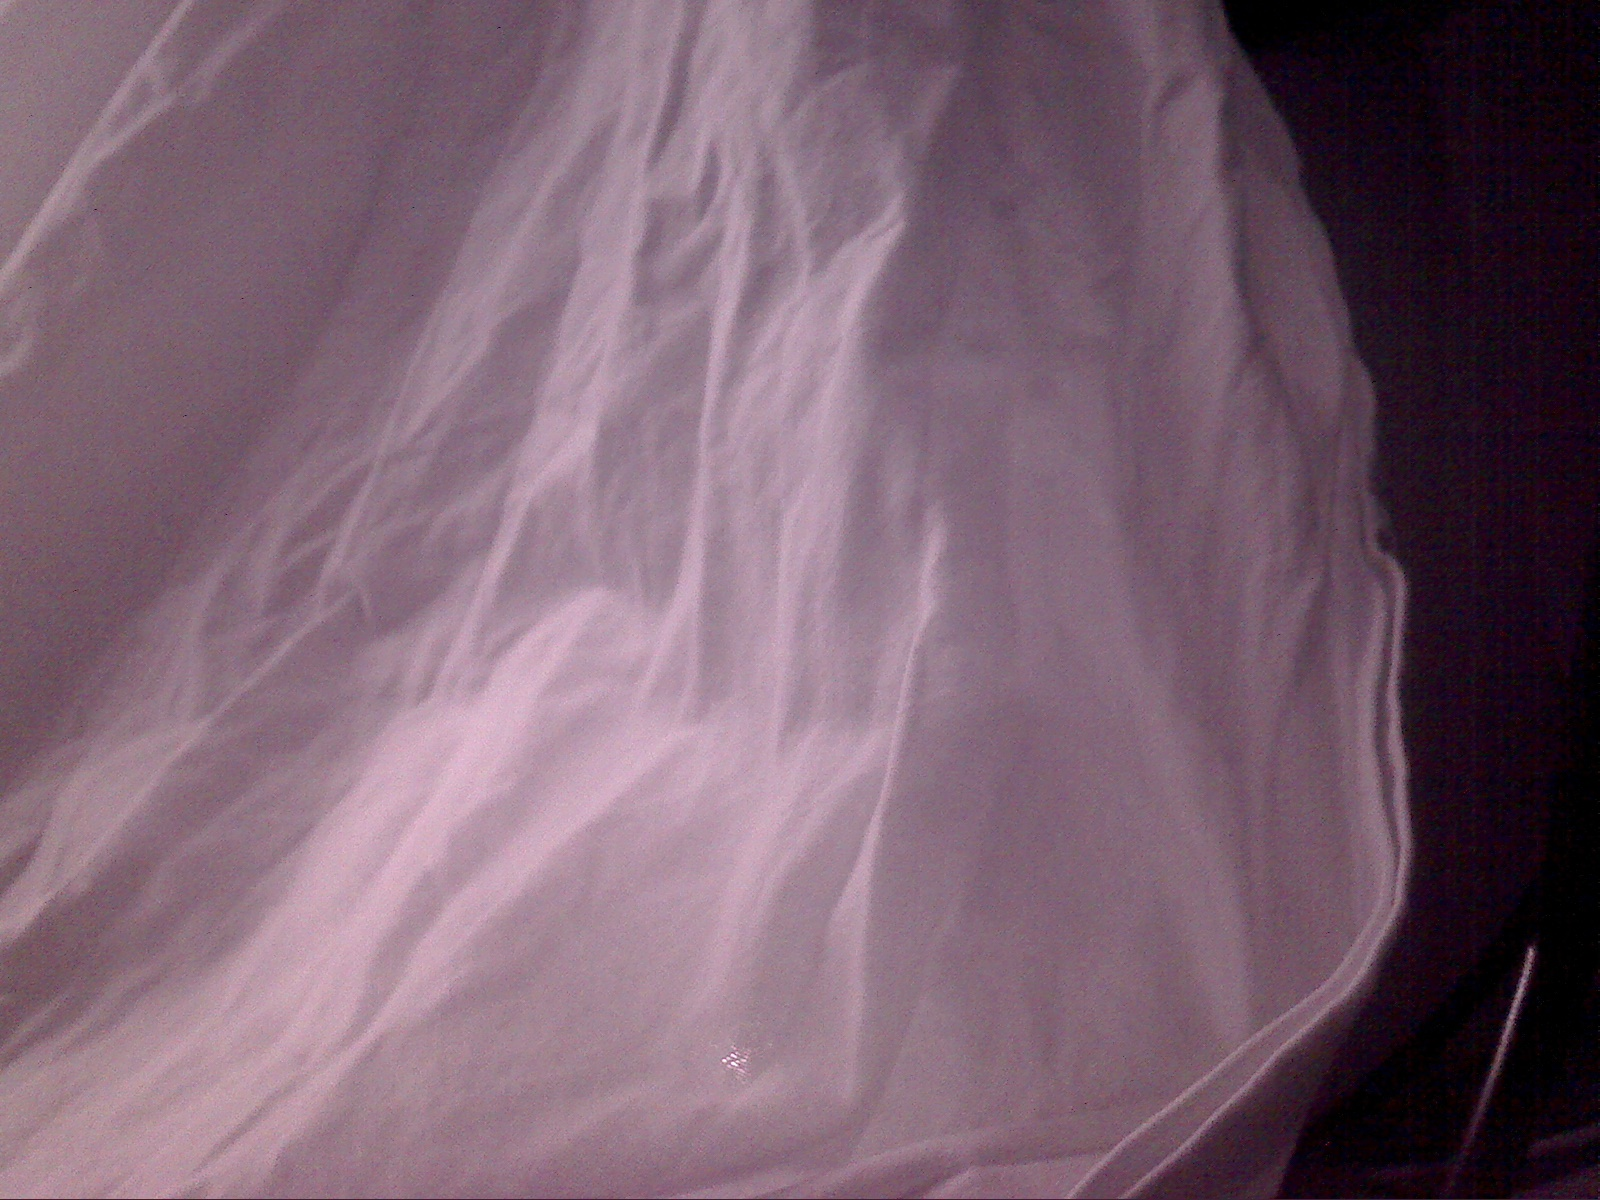
\includegraphics[width=1.00\textwidth]{Pictures/Theory/3mm.jpg} % Højre billede
\end{minipage} \\ % Captions og labels
\begin{minipage}[t]{0.45\textwidth}
\caption{5mm LED illuminates a sheet, that will later be used for projection.} % Venstre caption og label
\label{fig:5_mm_test}
\end{minipage} \hfill
\begin{minipage}[t]{0.45\textwidth}
\caption{3mm LED illuminates the same sheet.} % Højre caption og label
\label{fig:3_mm_led}
\end{minipage}
\end{figure}

Initially a broader strip of light was thought to be desirable, therefore a test was conducted where the LEDs had their lens sanded down in order to make the light less focussed. Figure \ref{fig:leds_sanded} shows an image where the LEDs in progression from left to right get more and more sanded down. As the figure illustrates the intensity of the light decreases as the LED-lens is sanded down. After conducting these tests,  it became clear that an unaltered LED performed better than the modified ones, providing a more intense illumination.

\begin{figure} [htbp]
\centering
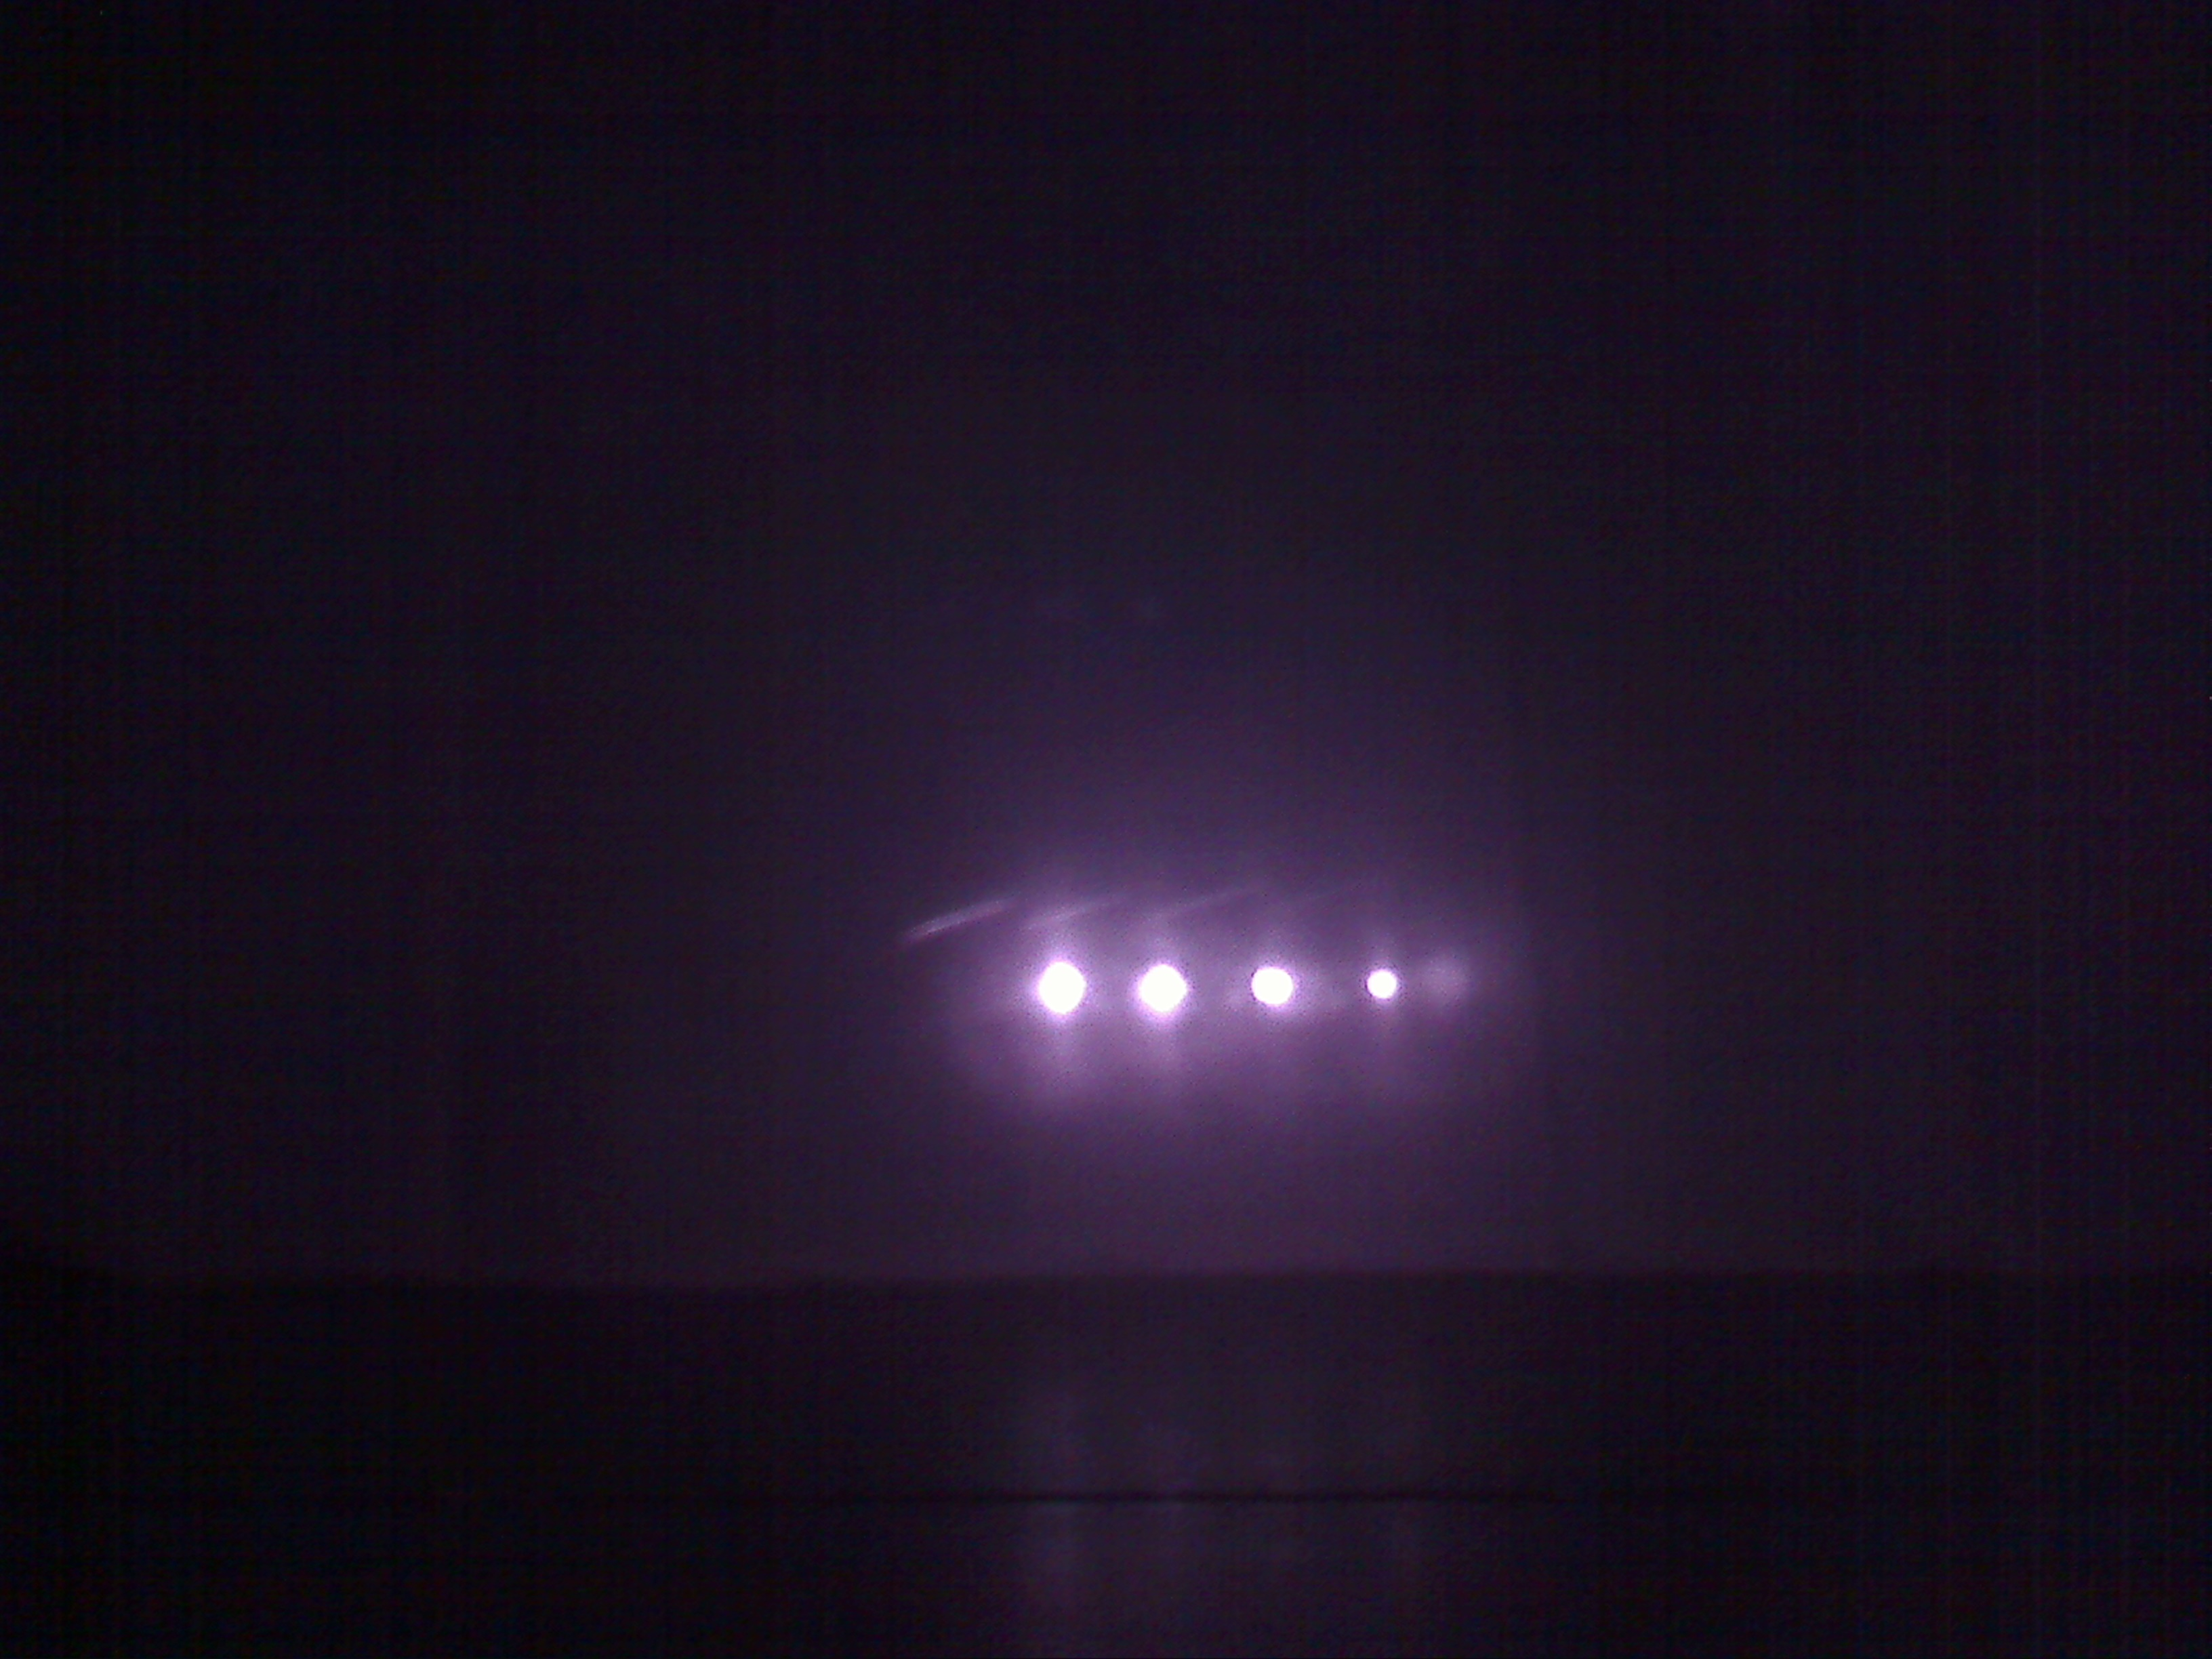
\includegraphics[width=1.00\textwidth]{Pictures/Theory/sanded_leds.jpg}
\caption{The LEDs have been sanded down in progressive order from left to right.}
\label{fig:leds_sanded}
\end{figure}

For ease of construction the LEDs were arranged into arrays of 8 LEDs connected in series, which in turn are connected in parallel. The LEDs have a forward voltage of 1.5V, which means that the power supply has to be able to supply at least 12V to power all 8 of them. Initially a small AC-DC power supply capable of supplying 12V at 600mA was used for testing purposes. However the total draw of a single LED array is 0,5A and for the project a total of 4 arrays were planned. The current far exceeded what could be supplied by the small AC-DC supply. Luckily the group managed to salvage a 300 watt computer power supply capable of supplying 12 volts at 8 amperes. After getting the power supply to work without being in a computer, terminals were soldered to LED-strips and the power supply allowing the LED-strips to plug into the power supply.

